%\documentclass[12pt]{article}
\documentclass[12pt]{scrartcl}
\title{ELEC 340 Assignment 3}
\nonstopmode
%\usepackage[utf-8]{inputenc}
\usepackage{graphicx} % Required for including pictures
\usepackage[figurename=Figure]{caption}
\usepackage{float}    % For tables and other floats
\usepackage{verbatim} % For comments and other
\usepackage{amsmath}  % For math
\usepackage{amssymb}  % For more math
\usepackage{fullpage} % Set margins and place page numbers at bottom center
\usepackage{paralist} % paragraph spacing
\usepackage{listings} % For source code
\usepackage{subfig}   % For subfigures
%\usepackage{physics}  % for simplified dv, and 
\usepackage{enumitem} % useful for itemization
\usepackage{siunitx}  % standardization of si units

\usepackage[bitstream-charter]{mathdesign}
\usepackage[T1]{fontenc}

\usepackage{tikz,bm} % Useful for drawing plots
%\usepackage{tikz-3dplot}
\usepackage{circuitikz}
\usepackage[ruled,vlined]{algorithm2e}
\usepackage[utf8]{inputenc}
\usepackage{tikz}


%%% Colours used in field vectors and propagation direction
\definecolor{mycolor}{rgb}{1,0.2,0.3}
\definecolor{brightgreen}{rgb}{0.4, 1.0, 0.0}
\definecolor{britishracinggreen}{rgb}{0.0, 0.26, 0.15}
\definecolor{cadmiumgreen}{rgb}{0.0, 0.42, 0.24}
\definecolor{ceruleanblue}{rgb}{0.16, 0.32, 0.75}
\definecolor{darkelectricblue}{rgb}{0.33, 0.41, 0.47}
\definecolor{darkpowderblue}{rgb}{0.0, 0.2, 0.6}
\definecolor{darktangerine}{rgb}{1.0, 0.66, 0.07}
\definecolor{emerald}{rgb}{0.31, 0.78, 0.47}
\definecolor{palatinatepurple}{rgb}{0.41, 0.16, 0.38}
\definecolor{pastelviolet}{rgb}{0.8, 0.6, 0.79}

\usepackage{pdfpages}
\usepackage{graphicx}
\usepackage{float}

%---------- Listings config


\usepackage{color}

\definecolor{dkgreen}{rgb}{0,0.6,0}
\definecolor{gray}{rgb}{0.5,0.5,0.5}
\definecolor{mauve}{rgb}{0.58,0,0.82}

\lstset{frame=tb,
  language=Java,
  aboveskip=3mm,
  belowskip=3mm,
  showstringspaces=false,
  columns=flexible,
  basicstyle={\small\ttfamily},
  numbers=none,
  numberstyle=\tiny\color{gray},
  keywordstyle=\color{blue},
  commentstyle=\color{dkgreen},
  stringstyle=\color{mauve},
  breaklines=true,
  breakatwhitespace=true,
  tabsize=3
}



\begin{document}

\begin{center}
	\hrule
	\vspace{.4cm}
	{\textbf { \large \scshape{ Práctica 1 - Regresión lineal y descenso según el gradiente}}}
\end{center}
{\ Javier Sáez \hspace{\fill} Aprendizaje Automático  \\
	\hrule

\section*{Ejercicio 1}

En este ejercicio, se implementará el algoritmo de descenso de gradiente y se aplicará
este sobre varias funciones con el objetivo de estudiar cómo afecta tanto el punto inicial 
como la tasa de aprendizaje $\eta$ a la solución que este algoritmo encuentra.\\

Lo primero que debemos hacer es recordar en qué consiste el algoritmo de descenso de gradiente,
 veámoslo en pseudocódigo:\\


\begin{algorithm}[H]
\SetAlgoLined
\KwResult{Mínimo local de una función}
 parametros: $\eta$, $f$, $max\_iteraciones$,$criterio\_parada$, $punto\_inicial$ \;

 $punto = punto\_inicial$ \;
 \While{No (Criterio de parada)}{
     $gradiente \leftarrow \nabla f(punto)$ \;
     $direccion \leftarrow - gradiente$ \;
     $punto \leftarrow punto - \eta \cdot direccion$
 }
 \caption{Descenso de gradiente}
\end{algorithm}

En la implementación en el lenguaje de programación escogido, \emph{python}, se podrá hacer todo el contenido de este bucle while en una única línea.
Sin embargo, se añadirá contenido extra al cuerpo de la función para que nos devuelva no solo el mínimo, sino también toda la sucesión de puntos
que se han ido obteniendo así como el número de iteraciones que se han dado. En este caso, consideraremos una iteración claramente como una actualización del punto mínimo
de la función. \\

\begin{lstlisting}[language=Python]
    def gradient_descent(eta,fun,grad_fun,maxIter,error2get,initial_point):
	    iterations = 0
	    w_t = initial_point
	    all_w = []
	    all_w.append(w_t)

	    while iterations < maxIter and fun(w_t) > error2get:
		    # All gradient descent in 1 line
		    w_t = w_t - eta*grad_fun(w_t)
		    all_w.append(w_t)
		    # sum iterations
		    iterations += 1
	

	    return np.array(all_w),w_t, iterations
\end{lstlisting}


\subsection*{Apartado 2}
Consideremos ahora la función

$$
E(u,v) = \left( u^3 e^{(v-2)} - 2v^2 e^{-u}\right)^2.
$$


Nuestra función $E$ es claramente derivable , así que procedemos a obtener sus derivadas parciales para poder aplicarle el algoritmo. Obtenemos que
$$
\frac{\partial E}{\partial u} = 2 \left( u^3 e^{(v-2)} - 2v^2 e^{-u}\right)\left( 3u^2 e^{(v-2)} + 2v^2 e^{-u}\right)
$$
y
$$
\frac{\partial E}{\partial v} = 2 \left( u^3 e^{(v-2)} - 2v^2 e^{-u}\right) \left( u^3 e^{(v-2)} - 4v e^{-u}\right).
$$

Tras definir una función para cada una de estas derivadas parciales y una para darnos el gradiente $\nabla E = \left(\frac{\partial E}{\partial u}, \frac{\partial E}{\partial v}\right)$ de $E$ en un punto
, podemos aplicar el algoritmo. Los parámetros de la ejecución son los siguientes:
\begin{itemize}
\item Tasa de aprendizaje $\eta = 0.1$.
\item Punto inicial $(u,v) = (1,1)$.
\item Condición de parada: Error $E$ inferior a $10^{-14}$ (esto está programado directamente en la función).
\item Máximo de iteraciones: prácticamente ilimitado ($10000000000$) para este primer ejercicio.
\end{itemize}

Tras la obtención del gráfico, se ha programado también una pequeña función que formatea la salida de algunos datos que pueden ser relevantes.
En particular, dada la propia función en un string, los parámetros del gradiente descendente y los resultados obtenidos del mismo,
esta función imprimirá estos parámetros, y los resultados obtenidos entre ellos el número de iteraciones y el punto final. Esta función se llama \lstinline{print_output_e1}
y el resultado sobre este problema es:

\begin{lstlisting}[language=bash]
    Gradiente descendente sobre la función: E(u,v) = (u^3 e^(v-2) - 2v^2 e^(-u))^2
    Punto inicial: [1. 1.]
    Tasa de aprendizaje: 0.1
    Numero de iteraciones:  10
    Coordenadas obtenidas: ( 1.1572888496465497 ,  0.9108383657484799 )
    Valor de la función de error en el mínimo :  3.1139605842768533e-15
\end{lstlisting}

Donde podemos ver las \textbf{iteraciones} que tarda el algoritmo en obtener por primera vez un valor de $E(u,v)$ por debajo de lo pedido, y además también
se observan las \textbf{coordenadas} en las que esto ocurre. Veamos cuál es la salida de dibujar la función y el mínimo por pantalla:

\begin{figure}[H]
  \centering
  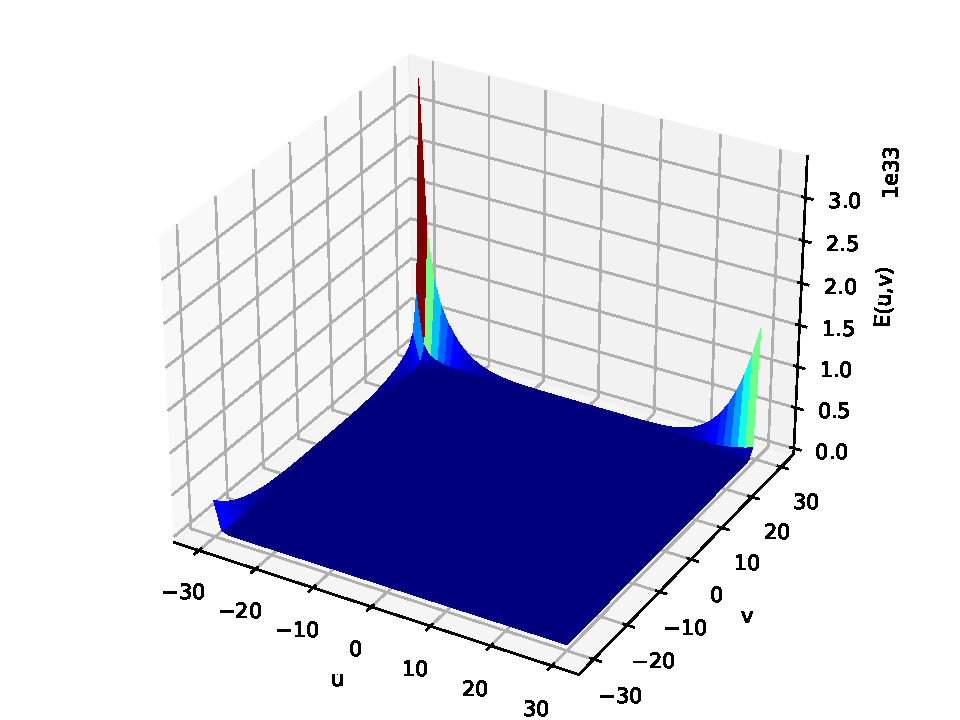
\includegraphics[scale=0.7]{media/E1-1.pdf}
  \caption{Mínimo local de la función}
\end{figure}

En este caso, el símbolo de estrella que simboliza el mínimo es muy difícilmente visible en el centro de la imagen. Esto es debido al rango dado para los ejes por defecto en el dibujo.
Vamos a dibujar ahora todos los puntos que ha ido obteniendo el algoritmo de descenso por el gradiente (para esto hemos devuelto una variable más en el código de la función) para ver cómo se ha ido buscando 
el mínimo de la función. El resultado es el siguiente:

\begin{figure}[H]
  \centering
  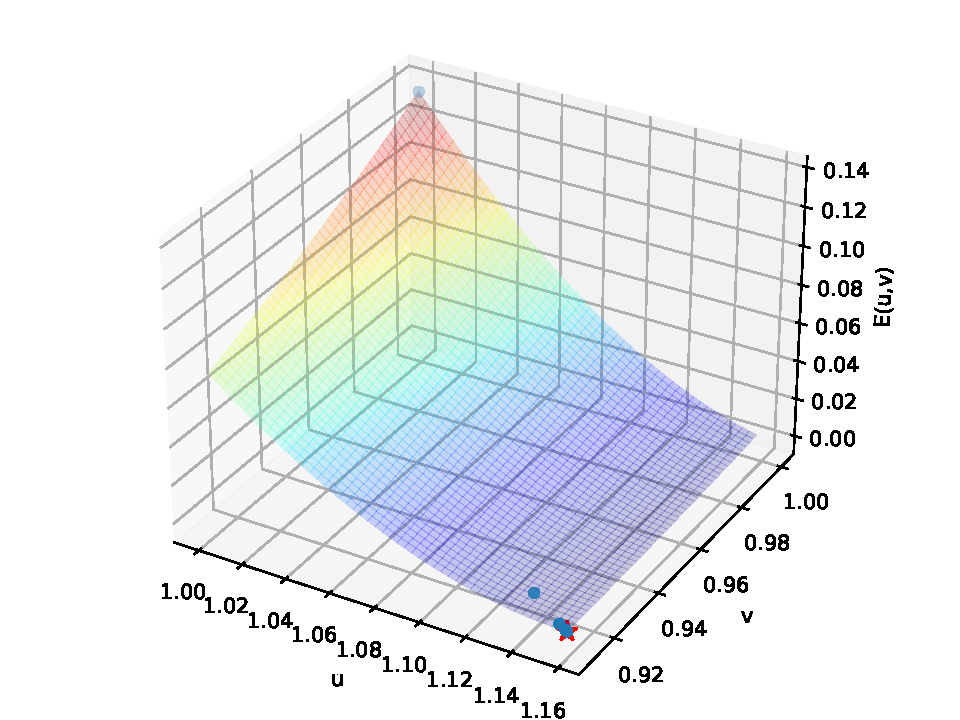
\includegraphics[scale=0.7]{media/E1-1-all.pdf}
  \caption{Mirada cercana al mínimo de la función}
\end{figure}

En esta imagen, obtenida usando el mismo código que la anterior salvo que el rango de dibujado de la superficie es únicamente el máximo de las coordenadas de los puntos que ha ido
obteniendo el algoritmo, se puede observar mucho mejor que se encuentra un mínimo local y como las iteraciones van buscando ese mínimo.

\subsection*{Apartado 3}

Vamos a considerar ahora una nueva función. Consideramos $f: \mathbb R^2 \to \mathbb R$ dada por:
\begin{equation}
f(x,y) = (x+2)^2 + 2(y-2)^2 + 2\sin(2\pi x) \sin(2\pi y). \label{eq:f}
\end{equation}
Por ser suma y producto de funciones derivables, es de nuevo una función derivable, cuyo gradiente viene dado por:
$$
\nabla f(x,y) = \Big( 2(x+2) + +4 \pi \cos(2 \pi x ) \sin (2 \pi y),\ 4 (y-2) + 4\pi \sin(2 \pi x) \cos (2 \pi y)\Big)
$$

La implementación de esta función en \emph{python} es la siguiente:\\

\begin{lstlisting}[language=Python]
  def f(x,y):
	  return (x + 2)**2 + 2*(y - 2)**2 + 2 * np.sin(2 * np.pi * x) * np.sin(2 * np.pi * y)

  def dfx(x,y):
	  return 2 * (x+2) + 4 * np.pi * np.cos(2* np.pi * x) * np.sin(2* np.pi * y)

  def dfy(x,y):
	  return 4 * (y-2) + 4 * np.pi * np.sin(2 * np.pi * x) * np.cos(2 * np.pi * y) 
\end{lstlisting}


Una vez implementado, volvemos a ejecutar el algoritmo de descenso según el gradiente en esta función. Esta vez, los parámetros son los siguientes:
\begin{itemize}
\item Punto inicial $(-1,1)$.
\item Tasa de aprendizaje $\eta = 0.01$.
\item Máximo de iteraciones $50$.
\item En este caso, suprimimos la condición del error a obtener, simplemente indicando que el error sea \lstinline{-math.inf}, y que se
realicen así las $50$ iteraciones.
\end{itemize}

El resultado de la ejecución es el siguiente:

\begin{lstlisting}[language=bash]
Gradiente descendente sobre la función: f(x,y) = (x+2)^2 + 2(y-2)^2 + 2 sin(2pi x) sin(2pi y)
Punto inicial: [-1.  1.]
Tasa de aprendizaje: 0.01
Numero de iteraciones:  50
Coordenadas obtenidas: ( -1.269064351751895 ,  1.2867208738332965 )
Valor de la función de error en el mínimo :  -0.3812494974381
\end{lstlisting}

Podemos ver el gráfico que nos genera la función utilizada en el ejercicio anterior para ver cómo desciende el valor de la función con las iteraciones.

\begin{figure}[H]
  \centering
  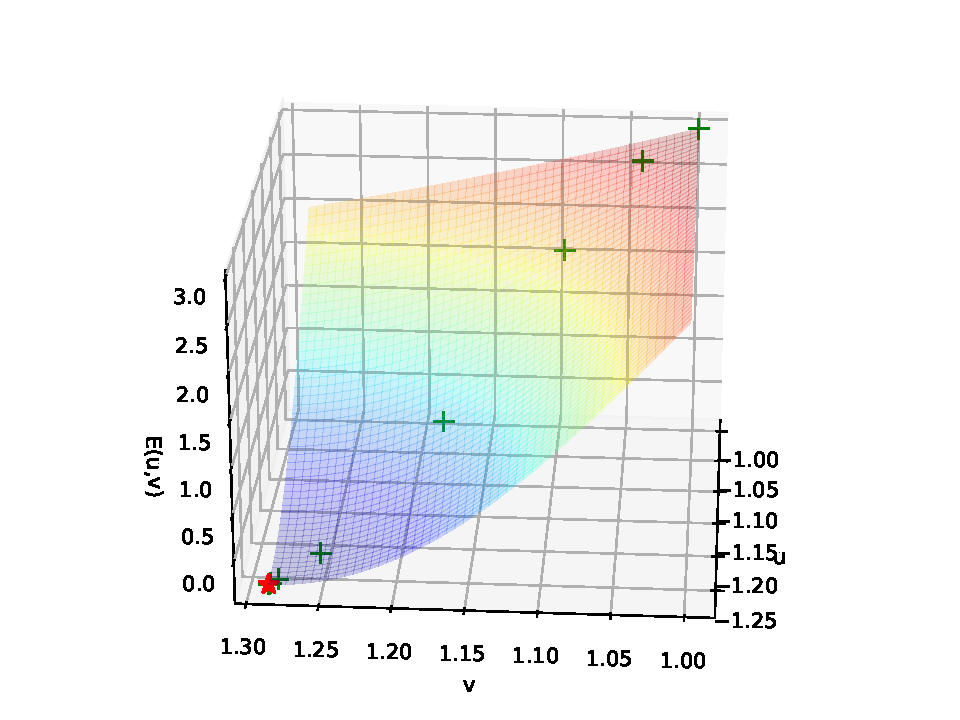
\includegraphics[scale=0.7]{media/E1-2-all-moved.pdf}
  \caption{Iteraciones en búsqueda del mínimo en $f(x,y)$ con $\eta = 0.01$.}
\end{figure}

Vemos como, igual que en el caso anterior, se encuentra el mínimo local en pocas iteraciones. Vamos a volver a repetir el experimento pero ahora usando $\eta = 0.1$, lo cual supone un cambio bastante grande. El resultado es el siguiente:

\begin{lstlisting}[language=bash]
Gradiente descendente sobre la función: f(x,y) = (x+2)^2 + 2(y-2)^2 + 2 sin(2pi x) sin(2pi y)
Punto inicial: [-1.  1.]
Tasa de aprendizaje: 0.1
Numero de iteraciones:  50
Coordenadas obtenidas: ( -2.9604132205400098 ,  0.5733549488050332 )
Valor de la función de error en el mínimo :  4.774050376444264
\end{lstlisting}

Se puede ya observar como el valor encontrado esta vez es muy diferente, además de ser claramente superior en su valor de $f$. 
Esto es debido a que al ser la tasa de aprendizaje $\eta$ mucho mayor, los saltos que se dan en la dirección opuesta a la del gradiente son de gran tamaño y se salta en la función a sitios en los que los mínimos son
diferentes que en el punto inicial, y el gradiente puede tener además una dirección completamente diferente a la que tenía en el punto anterior, por lo que la dirección de la nueva iteración puede cambiar mucho de nuevo. Vemos el resultado de todos los saltos que
da el algoritmo de descenso según el gradiente:

\begin{figure}[H]
  \centering
  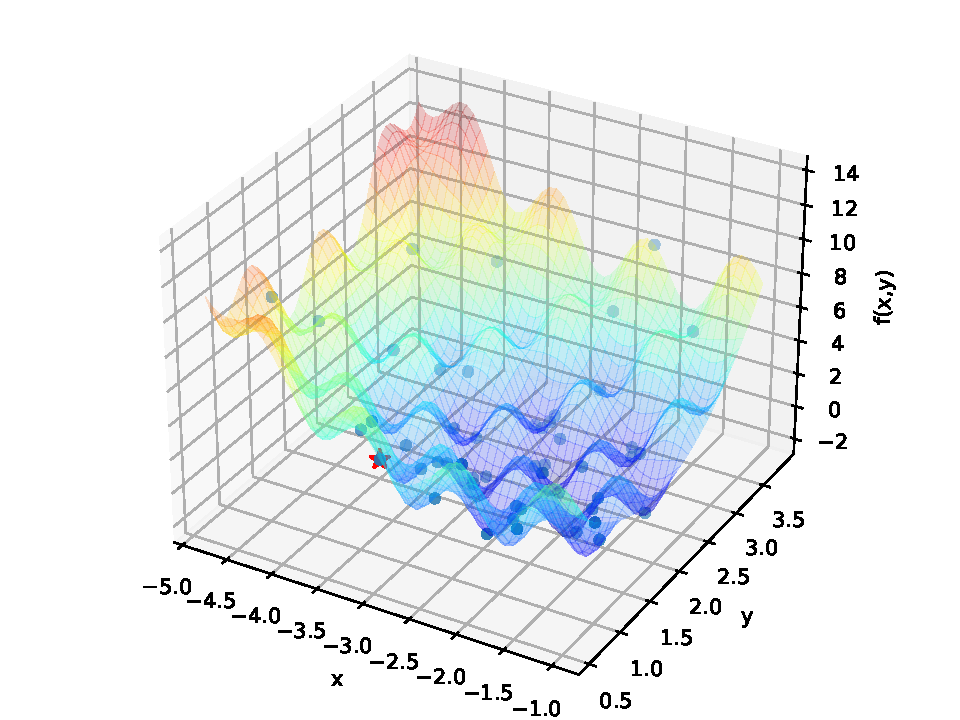
\includegraphics[scale=0.7]{media/E1-2-loweta-all.pdf}
  \caption{Iteraciones en búsqueda del mínimo en $f(x,y)$ con $\eta = 0.1$.}
\end{figure}

Vamos a ver qué ocurre cuando tomamos varios puntos diferentes y ejecutamos el algoritmo con $\eta = 0.01$, para tratar de que los saltos de dirección no sean muy grandes. Vamos a generar una tabla con el mínimo obtenido de cada uno de los siguientes puntos:
$(-0.5,-0.5),(1,1),(2.1,-2.1),(-3,3),(-2,2)$ y veamos qué valores alcanzan desde cada uno como mínimos locales.

\begin{table}[]
  \begin{tabular}{llll}
  Punto inicial   & Mínimo $(x,y)$ contrado       & Imagen en el mínimo $f(x,y)$ & Iteraciones \\
  {[}-0.5  0.5{]} & {[}-0.78365509  0.81314011{]} & 2.4931912832664618           & 50          \\
  {[}1. 1.{]}     & {[}0.67743878 1.29046913{]}   & 6.4375695988659185           & 50          \\
  {[} 2.1 -2.1{]} & {[} 0.14880583 -0.0960677 {]} & 12.490971442685037           & 50          \\
  {[}-3.  3.{]}   & {[}-2.73093565  2.71327913{]} & -0.38124949743809955         & 50          \\
  {[}-2.  2.{]}   & {[}-2.  2.{]}                 & -4.799231304517944e-31       & 50         
  \end{tabular}
\end{table}


Como vemos, cada mínimo es diferente según el punto de inicio. Esto es debido a que el mínimo local encontrado depende del punto inicial. Podemos ver los diferentes mínimos encontrados en la siguiente imagen generada:

\begin{figure}[H]
  \centering
  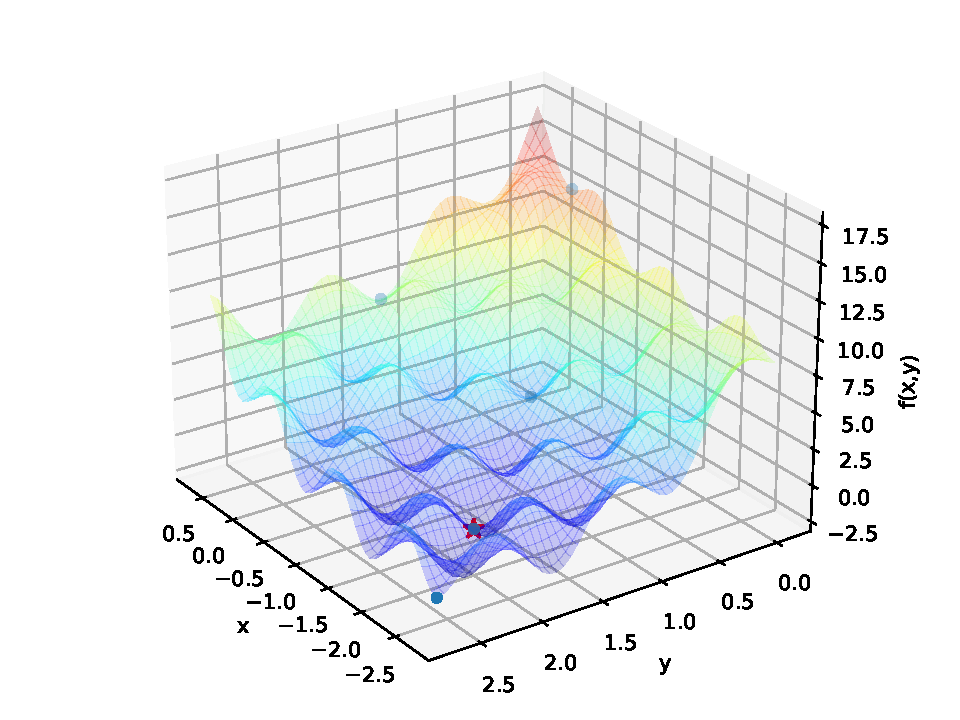
\includegraphics[scale=0.7]{media/E1-2-minimums-moved.pdf}
  \caption{Dependencia del punto inicial en el algoritmo de descenso según el gradiente.}
\end{figure}

Como se puede observar, el algoritmo está encontrando mínimos locales, que según el punto en el que hayamos iniciado son diferentes, lo cual nos muestra esta dependencia fuerte del del punto inicial que se utilice para comenzar el algoritmo, ya que el algoritmo
como sabemos acaba encontrando mínimos locales.


\subsection*{Conclusiones}

Terminamos el ejercicio haciendo una pequeña conclusión sobre los resultados obtenidos. Usando la función $f(x,y)$ definida en \eqref{eq:f} , nos ha permitido ver como partiendo desde un mismo punto y usando diferentes tasas de aprendizaje $\eta$, los mínimos que se obtienen
pueden ser radicalmente distintos. Esto es debido a que el cambio que hacemos en el punto depende de esta tasa de aprendizaje y si esta crece, el salto que da el punto en cada iteración puede hacer que el algoritmo vaya \emph{saltando} entre diferentes mínimos locales.

Además de eso, hay que comentar que el punto inicial es también muy relevante en la búsqueda del mínimo global, pues dependiendo de dónde comencemos, podemos quedarnos atrapados en un mínimo local y que nuestro algoritmo no encuente el mínimo global. Aunque ya hemos visto un ejemplo claro
con la función $f(x,y)$, podemos ver un ejemplo mucho más sencillo de que esto puede pasar incluso con funciones $f:\mathbb R \to  \mathbb R$, como en el siguiente ejemplo:

\begin{figure}[H]
\centering
\begin{tikzpicture}[scale=0.8]

  \definecolor{xdxdff}{rgb}{0.49019607843137253,0.49019607843137253,1}
  \draw[step=1cm,gray,very thin] (-1.99,-0.5) grid (3.99,0.5);
  
\draw [fill=xdxdff] (-1,0) circle (2.5pt);
\draw[color=xdxdff] (-1.3,-0.3) node {$A$};
\draw [fill=xdxdff] (3,0) circle (2.5pt);
\draw[color=xdxdff] (3.3,-0.3) node {$B$};
  \draw[scale=1, domain=-1.1:3.2, smooth, variable=\x, red] plot ({\x}, {(\x)^(4) - 5*(\x)^(3) + 5*(\x)^(2) +5*(\x) -6 });
\end{tikzpicture}
\caption{Dos mínimos locales en $f(x) = x^4 - 5 x^3 + 5 x^2 + 5 x - 6 $}
\end{figure}

Vemos que tenemos dos mínimos locales y uno global, pero si nuestro $\eta$ no es suficientemente grande, empezando por los puntos marcados $A$ y $B$, podríamos obtener como puntos mínimos dos diferentes y en este caso uno sería el correcto (al que llegamos desde $A$) y el otro no.

Por estos dos motivos principales, concluimos que la verdadera dificultad de encontrar el mínimo global está en encontrar un punto inicial adecuado así como una tasa de aprendizaje que no sea ni demasiado grande y nos haga salirnos de esos mínimos, ni demasiado pequeña y nos fuerce
a realizar un número de iteraciones muy grande para encontrar ese mínimo global.

\end{document}
